\chapter{Definición de las instancias: archivo de red y tráfico}
\label{cap:instancias}

\section{Definición de la zona de simulación: el archivo de red}
\label{def_zona_sim_archivo_red}

\subsection{Generación y conversión}
\label{gen_conv}

La zona de la rotonda del Padre Anchieta ha sido extraída de \textit{OpenStreetMap} (OSM), servicio gracias al cual ha sido posible obtener una representación fiel y bastante completa de la rotonda y las vías conexas. OSM permite seleccionar una zona del mapa y descargarla en formato \texttt{.osm}.

Aunque inicialmente se había seleccionado una zona considerable grande de la rotonda (incluyendo, por ejemplo, calles de la zona de la Av. Trinidad, como la Obispo Rey Redondo; así como vías de la zona del Coromoto), finalmente se seleccionó una zona que únicamente abarca la rotonda, las entradas y salidas y el tramo de la TF-5 que pasa por debajo, incluyendo las entradas y salidas de la autopista. Esto se debe a que los datos de tráfico disponibles se circunscriben únicamente a las zonas mencionadas, por lo que no se podría haber simulado otras vías conexas sin perder fiabilidad en la simulación (al tener que aproximar los datos de los vehículos que circulan por dichas vías, en vez de contar con datos empíricos).

OSM ofrece los datos en formato <<.osm>>; sin embargo, los archivos de red legibles por SUMO y las demás herramientas del simulador siguen un formato XML con extensión \texttt{.net.xml}. Para realizar la conversión se empleó una de las herramientas que viene con el simulador, denominada \texttt{NETCONVERT}. Esta herramienta está específicamente destinada a importar archivos redes viales de diferentes fuentes para generar redes viales que puedan ser utilizadas por otras herramientas~\cite{noauthor_netconvert_nodate} (como SUMO, NetEdit, etc.).

% El comando empleado para ejecutar \texttt{NETCONVERT} fue el siguiente:

% \begin{lstlisting}[breaklines=true]
% netconvert --type-files osmNetconvert.typ.xml,osmNetconvertPedestrians.typ.xml --osm-files <Archivo OSM> --output-file <Nombre del archivo de salida> --geometry.remove --roundabouts.guess --ramps.guess --junctions.join --tls.guess-signals --tls.discard-simple --tls.join --no-turnarounds.except-deadend --crossings.guess --osm.all-attributes --sidewalks.guess
% \end{lstlisting}

Los archivos \texttt{xml} que se pasan al comando vienen predefinidos en el pack de herramientas de SUMO, y sirven principalmente para definir el modo en que se clasificarán las vías en el momento de convertirlas (por ejemplo, qué vías se clasificarán como calles o autopistas, con qué velocidad, etc.), así como la adición de aceras y pasos peatonales. El resto de \textit{flags} señalan a \texttt{NETCONVERT} cómo debe realizar la conversión (por ejemplo, pidiendo que infiera las intersecciones, los carriles de aceleración y desaceleración de las autopistas, etc.).

El archivo que obtenemos como resultado del proceso de conversión es con el cual podemos empezar a trabajar con SUMO y las herramientas que trae consigo.

\subsection{Limpieza}

\subsubsection{Intersecciones}

Pese a que \texttt{NETCONVERT} hace un excelente trabajo generando el archivo de red, todavía es necesario realizar pequeños cambios antes de que pueda llevarse a cabo la simulación. Esto se realizó mediante \texttt{NETEDIT}, otra de las herramientas que viene en el paquete de SUMO, y que está orientada a editar archivos de red mediante una GUI, ya sea para modificar las vías (o los metadatos de estas), la forma de las intersecciones, los semáforos, el orden de preferencias en las vías, y toda una serie de funcionalidades relacionadas~\cite{noauthor_netedit_nodate}. El trabajo principal que se ha realizado en este aspecto tiene que ver con la forma de las intersecciones. 

La manera en que dos vías se conectan en SUMO (y, por extensión, en \texttt{NETEDIT}) viene determinada por el Modelo de Intersección de Vías de SUMO~\cite{erdmann_sumos_2014}. Explicado superficialmente, en SUMO la red de vías se representa mediante un grafo. Una intersección consiste en un nodo \textit{de entrada} y otro \textit{de salida} (donde un nodo representa una vía con un identificador concreto, y que sea de entrada o de salida implica de dónde viene y hacia donde va un vehículo). Así pues, un carril de entrada puede tener varios carriles de salida posibles (o sea, varios destinos que puede tomar un vehículo en una intersección).

Bien, dentro de esta intersección existen los denominados <<carriles internos>>, que conectan los nodos de entrada con los de salida y permiten especificar con exactitud por donde deben circular los vehículos en la intersección. Estos carriles internos son calculados automáticamente por \texttt{NETCONVERT}, pero a veces falla o los calcula de una manera inexacta, lo que provoca que algunas intersecciones proporcionadas por el conversor no representen con fidelidad la  intersección real.

Asimismo, es muy importante configurar bien las intersecciones puesto que son necesarias para añadir los semáforos y configurarlos adecuadamente en función de las vías que vaya a regular; situación que también se da para los pasos de peatones.

La mayoría del trabajo de limpieza consistió, pues, en procurar la exactitud de las intersecciones de las vías de entrada y salida de la rotonda. Esto es posible modificando la forma de estas en \texttt{NETEDIT}; pero, por desgracia, es un trabajo en gran parte tedioso y a veces frustrante, puesto que la manera en que están definidas estas intersecciones es mediante un conjunto de puntos (que encierran la zona por la que pasan los carriles internos, como se ve en la figura~\ref{fig:interseccion3}). 

\begin{figure}[ht]
    \centering
    \begin{subfigure}[t]{.30\textwidth}
      \centering
      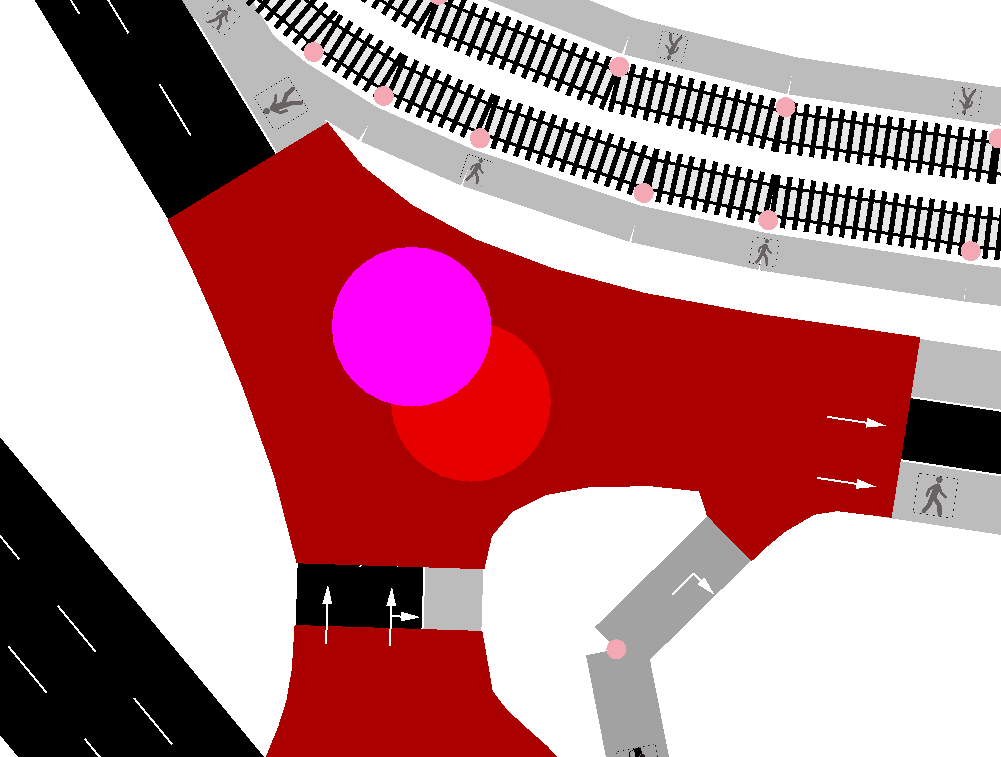
\includegraphics[width=\textwidth]{report/images/interseccion1.png}
      \caption{Forma de la intersección (señalada en rojo).}
      \label{fig:interseccion1}
    \end{subfigure}
    \hfill
    \begin{subfigure}[t]{.30\textwidth}
      \centering
      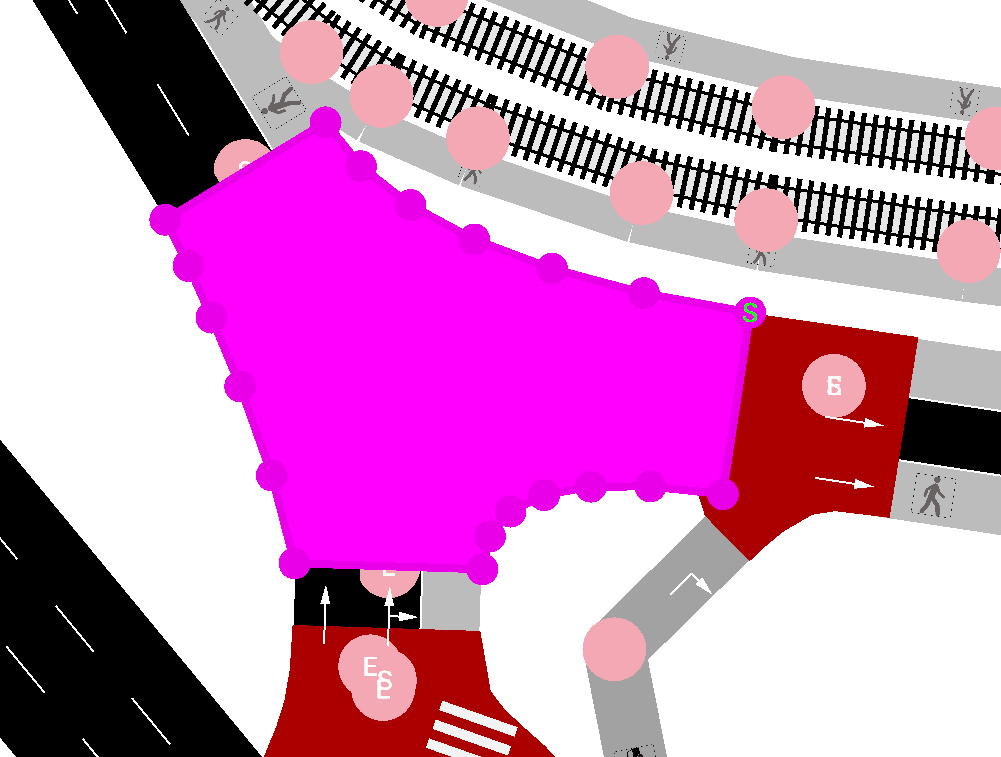
\includegraphics[width=\textwidth]{report/images/interseccion2.png}
      \caption{Modo de edición de la intersección (en violeta). Se aprecian los puntos que definen la forma.}
      \label{fig:interseccion2}
    \end{subfigure}%
    \hfill
    \begin{subfigure}[t]{.30\textwidth}
      \centering
      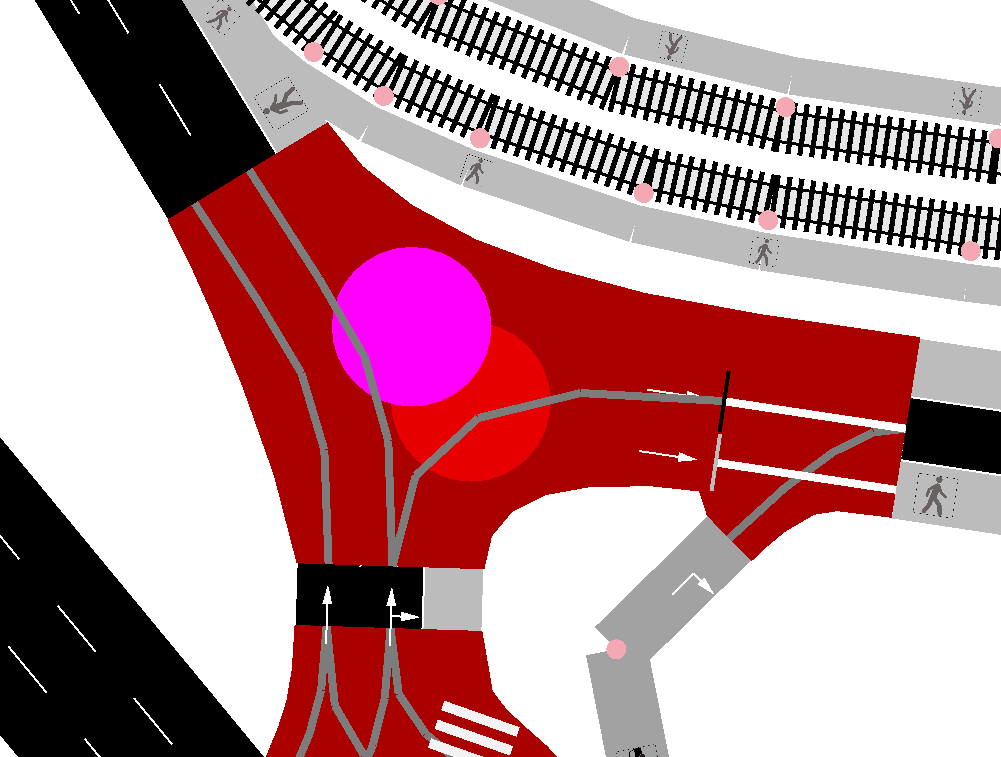
\includegraphics[width=\textwidth]{report/images/interseccion3.png}
      \caption{Carriles internos (señalados en gris). La forma de estos depende de la forma de la intersección.}
      \label{fig:interseccion3}
    \end{subfigure}
    \caption{Representación de las intersecciones en \texttt{NETEDIT}.}
    \label{fig:interseccion}
\end{figure}

Además, cabe mencionar que \texttt{NETEDIT}, en determinadas circunstancias o al intentar algunas modificaciones en concreto, ha llegado a cerrarse de forma inesperada debido a un error interno del programa, resultando además que se perdía todo el trabajo realizado hasta el momento, por lo que había que empezar de nuevo.

\subsubsection{Vías mal priorizadas}

Para señalar la prioridad de una vía sobre otra, SUMO asigna un \textit{valor de prioridad} en función del tipo de vía que sea, de acuerdo con una clasificación que también emplea \textit{OpenStreetMap}. Por ejemplo, una autopista tiene prioridad sobre las carreteras primarias, estas sobre las carreteras secundarias, estas sobre las calles urbanas, etc. 

Durante el proceso de conversión es posible que algunas vías no estén señaladas o priorizadas adecuadamente, dando lugar a que los ceda el paso se produzcan por vías a las que en realidad les corresponde la prioridad en una intersección. Este fue el caso de algunas entradas de la rotonda.

Hay una \textit{flag} que se puede añadir al comando \texttt{NETCONVERT} mencionado en la sección~\ref{gen_conv} que se denomina \texttt{--roundabouts.guess}. Esta \textit{flag} permite que, durante el proceso de conversión, se detecten automáticamente las rotondas y se ajusten las prioridades de acuerdo con la norma general: las vías de la rotonda en sí tienen prioridad sobre las vías de entrada. Sin embargo, al ser un método heurístico, es posible que falle y es el caso ante el cual nos encontramos.

Por suerte, corregirlo no es particularmente complicado. Basta con reducir el valor de prioridad de la vía de entrada con respecto al de la rotonda y problema solucionado.

\subsubsection{Vías mal representadas}

Este es un caso bastante particular y tiene que ver con la salida de la TF-5, en dirección norte, que permite incorporarse a la rotonda de Padre Anchieta (representado en la figura \ref{fig:salida-tf5-norte}). 

\begin{figure}[ht]
    \centering
    \begin{subfigure}[t]{0.48\textwidth}
      \centering
      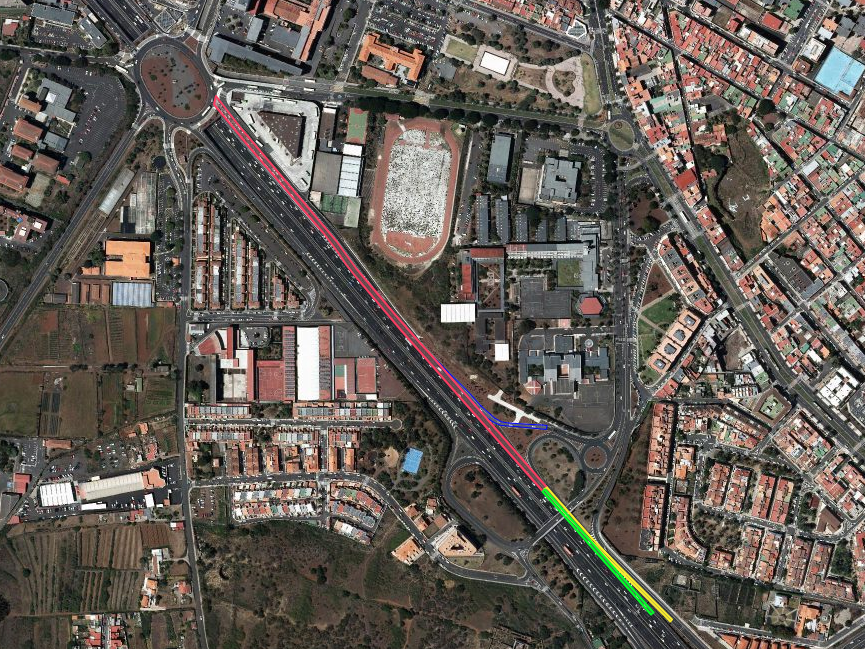
\includegraphics[width=\textwidth]{report/images/salida-tf5-norte-lejos_.png}
      \caption{La salida de la TF-5 (dir. norte) a la rotonda de Padre Anchieta vista desde lejos.}
      \label{fig:salida-tf5-norte-lejos}
    \end{subfigure}
    \hfill
    \begin{subfigure}[t]{0.48\textwidth}
      \centering
      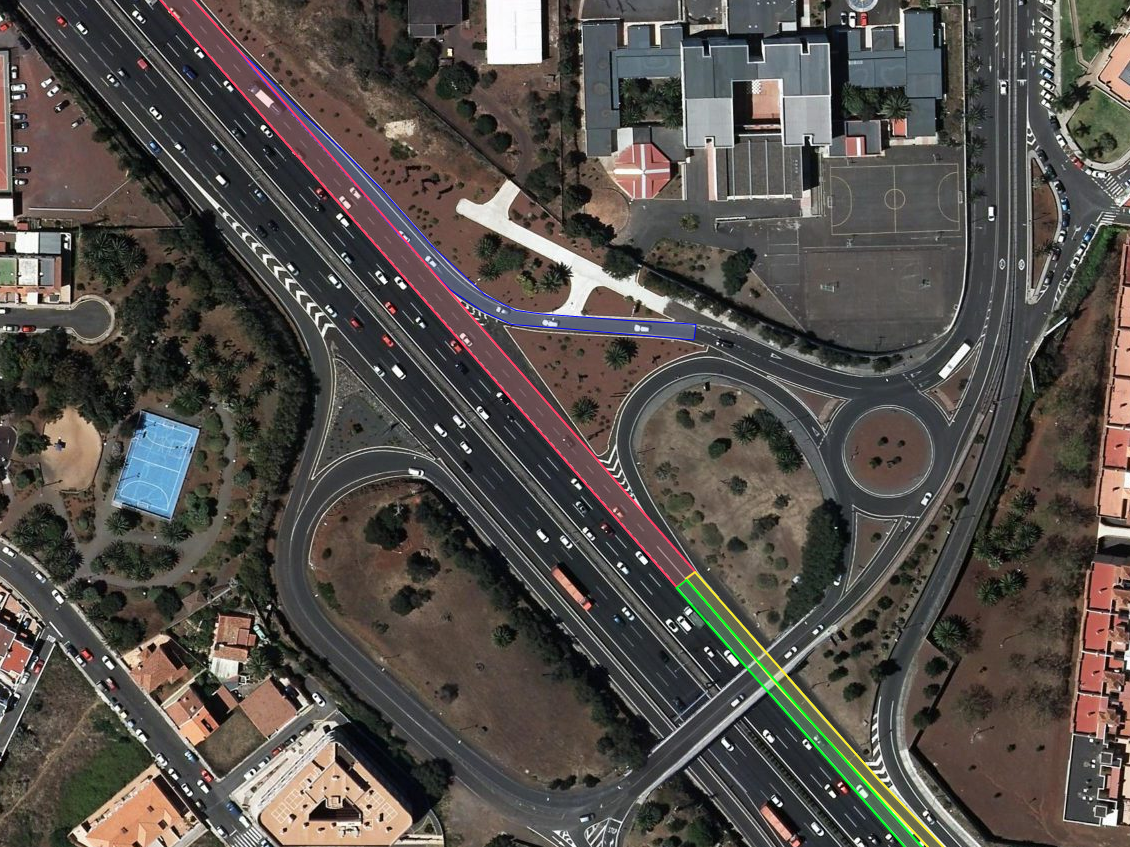
\includegraphics[width=\textwidth]{report/images/salida-tf5-norte-cerca_.png}
      \caption{La misma vista, desde cerca. Permite apreciar los distintos carriles que dan lugar o se incorporan a la salida en cuestión.}
      \label{fig:salida-tf5-norte-cerca}
    \end{subfigure}%
    \caption{La zona roja representa la vía de doble carril (el de la izquierda permite la incorporación a la autopista y también ir a la rotonda de Padre Anchieta, mientras que el derecho permite ir a la rotonda únicamente). La azul se corresponde con la carretera proveniente del IES Viera y Clavijo. El carril verde es el proveniente de la autopista, y el amarillo el proveniente de la rotonda que está por debajo de la autopista. Los tres dan lugar a la vía representada por la zona roja.}
    \label{fig:salida-tf5-norte}
\end{figure}

Bien, la vía representada zona roja (figura~\ref{fig:salida-tf5-norte-cerca}) permite ir a la rotonda o incorporarse a la autopista. Esta incorporación a la TF-5 tiene sentido para los vehículos que vienen de la zona azul o la amarilla. También tendría sentido para los vehículos que provinieran de la autopista (zona verde) que pese a haber tomado la salida deseen reincorporarse a la autopista.

Este comportamiento es el correcto; sin embargo, durante el proceso de conversión \texttt{NETCONVERT} se equivocó y generó un archivo de red que no permitía que los vehículos provenientes de las zonas mencionadas pudieran incorporarse a la TF-5 en dicho lugar (figura~\ref{fig:netedit-tf5-norte-mal}), lo que provocaba que tuvieran que pasar por la rotonda de Padre Anchieta y tomar desde ahí la salida en dirección a la TF-5. Tal comportamiento es indeseable y se corrigió.

\begin{figure}[ht]
    \centering
    \begin{subfigure}[t]{0.48\textwidth}
      \centering
      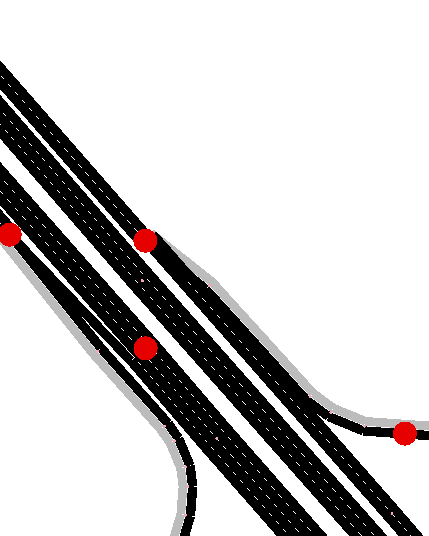
\includegraphics[width=\textwidth]{report/images/netedit-tf5-norte-mal.png}
      \caption{Generación inicial. Véase cómo no es posible la incorporación a la autopista desde los dos carriles que aparecen más a la derecha, que separados de los tres que están en medio (TF-5 dirección norte).}
      \label{fig:netedit-tf5-norte-mal}
    \end{subfigure}
    \hfill
    \begin{subfigure}[t]{0.48\textwidth}
      \centering
      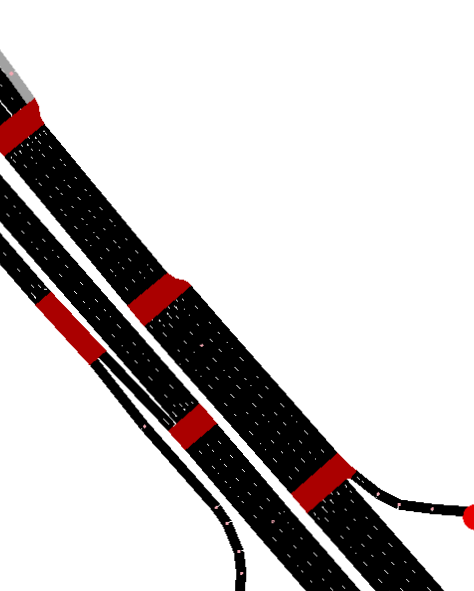
\includegraphics[width=\textwidth]{report/images/netedit.-tf5-norte-bien.png}
      \caption{Modificación realizada. Ahora los vehículos pueden incorporarse a la autopista, pero también los de la autopista pueden tomar la salida más adelante de lo que deberían.}
      \label{fig:netedit-tf5-norte-bien}
    \end{subfigure}%
    \caption{Cambios realizados en la salida de la TF-5 (dir. norte) que va a la rotonda del Padre Anchieta.}
    \label{fig:netedit-tf5-problema}
\end{figure}

Sin embargo, por limitaciones de SUMO, actualmente no es posible establecer carriles con prohibición de cambio asimétrica (como es el caso de la zona roja que se menciona antes): es decir, actualmente no se puede implementar un cambio de carril de modo que sea posible incorporarse a la autopista pero no sea posible realizar la acción inversa. Ello implica que con la modificación realizada para solucionar el problema los vehículos que vayan por la autopista podrán tomar la salida mucho más adelante de lo que en realidad pueden hacerlo (figura~\ref{fig:netedit-tf5-norte-bien}). No obstante, esta solución, aunque imperfecta, es mejor que impedir la incorporación a la TF-5 por los motivos mencionados en el párrafo anterior.

\subsubsection{Otras modificaciones}

Mencionadas las modificaciones más sustanciales, en el archivo de red también se han realizado otras modificaciones menores como la forma de algunas vías (especialmente las vías de la rotonda en sí), que han sido retocadas para que sean más fieles a la realidad; la adición de pasos de peatones, la adición de aceras cuando era necesario y la supresión cuando eran aceras innecesarias o no se correspondían con la realidad, la configuración de los semáforos (de la que se hablará en su propia sección), la corrección de algunas conexiones que permitían giros prohibidos, etc.

\section{Definición de los vehículos y las rutas: el archivo de tráfico}

El principal objetivo a la hora de generar el tráfico y los peatones era hacerlo para una hora de simulación, de modo que dicha hora fuera punta (por ejemplo, a las 8:00 o las 14:00).

En este sentido, varios enfoques han sido tomados en cuenta, resultando al final como ganador la generación de tráfico en función de un algoritmo de maximización del flujo de red, con datos empíricos de aforadores de tráfico provistos por el Cabildo de Tenerife, gracias a un estudio que realizó la entidad en noviembre de 2019 en la rotonda de Padre Anchieta. 

Sin embargo, es relevante mencionar otros enfoques que en durante el desarrollo de este proyecto se tomaron en cuenta, dado que los datos del Cabildo se obtuvieron más adelante durante la fase de desarrollo de este trabajo.

\subsection{Enfoque estocástico}
\label{enfoque_estocastico}

Este enfoque es el más sencillo. Consiste en generar los datos de tráfico y de peatones de forma aleatoria, tanto en flujo como en rutas. SUMO cuenta con una herramienta para hace precisamente esto, \texttt{randomTrips.py}~\cite{noauthor_randomtripspy_nodate}, un script de Python que, con un archivo de red como entrada, permite generar sendos archivos de tráfico y peatones aleatorios.

Las desventajas que plantea este método saltan a la vista: los datos de tráfico generados muy probablemente no se correspondan con la realidad. Esto plantea un problema serio a la hora de obtener una simulación fiel, puesto que los datos de circulación en una situación como la actual pueden afectar sensiblemente al resultado final de la simulación y, en consecuencia, no se podría determinar con fiabilidad si los semáforos son una adición útil o no (que al final es el objetivo último de este trabajo).

A falta de datos de tráfico, este enfoque parece el más aceptable. Sin embargo, el Cabildo de Tenerife publica anualmente un estudio de las intensidades de tráfico en las carreteras de Tenerife~\cite{rodriguez_hernandez_intensidades_2019}. Este estudio no contiene los datos de los aforadores de la rotonda de Padre Anchieta que se mencionaban antes, pero sí contiene la intensidad media diaria (IMD) anual de algunas vías que conectan con la rotonda. La IMD anual de define como el número de vehículos que pasan a través de una sección fija de la carretera dividido entre 365.

Por ejemplo, de las vías que nos interesan el informe contiene los datos de la IMD anual de la TF-5, de la TF-24 (la carretera de La Esperanza) y de la TF-263 (la carretera de Geneto). También tienen datos de la TF-265 (Camino de San Francisco de Paula) pero dicha carretera no conecta directamente con la rotonda, sino que lo hace con la Av. Astrofísico Francisco Sánchez, que sí es una vía de que entra y sale de la rotonda.

Estos datos son extremadamente débiles para inferir el tráfico en una hora particular, sobre todo si queremos el caso de la hora punta de las vías en cuestión. Y eso sin mencionar de que todavía nos faltarían datos de otras vías. Ello nos lleva a plantear el siguiente método.

Sin embargo, este sí fue el enfoque empleado para generar los peatones, puesto que no se dispone de ningún dato sobre los movimientos de las personas que atraviesan los pasos de peatones de las vías de la rotonda.


\subsection{Enfoque de inundación}


\begin{wrapfigure}{L}{5.5cm}
    \centering
    % \captionsetup{width=.8\linewidth}
    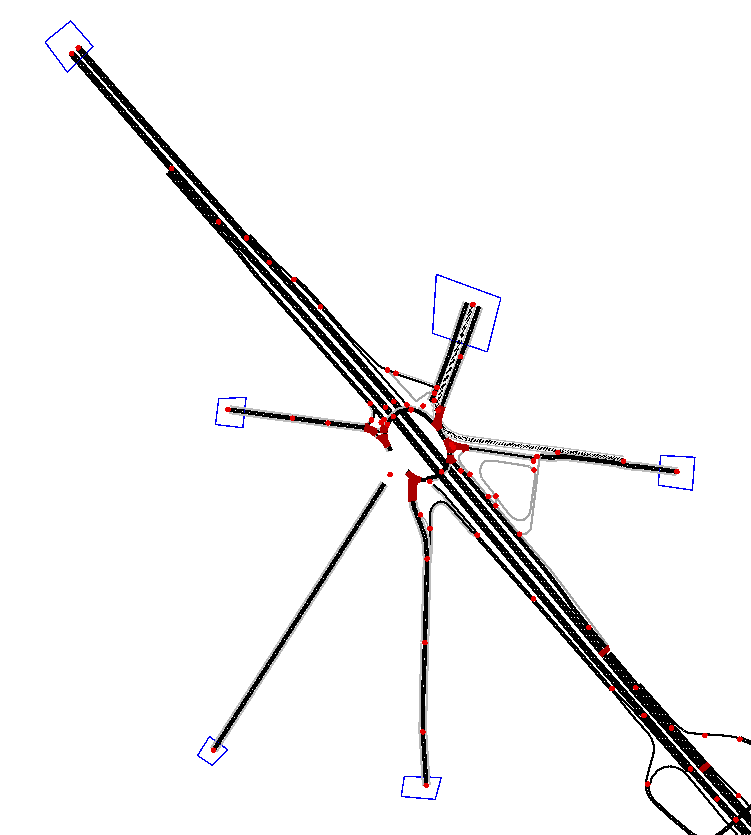
\includegraphics[width=\linewidth]{report/images/taz.png}
    \caption{Las TAZ aparecen delimitadas por las líneas azules.}
    \label{fig:taz}
\end{wrapfigure}


A falta de datos para generar el tráfico, un enfoque interesante residía en generar el tráfico de modo que se lleva al límite el aforo de las vías de la rotonda; es decir, propiciando que circulara el máximo tráfico posible por todas las vías. Este enfoque, aunque en determinados casos resulte irreal, en cierta medida no es tan diferente de lo que sucede en realidad, puesto que en horas punta la rotonda de Padre Anchieta sufre de colas en todas las entradas (en las entradas desde autopista, tanto del norte como del sur, en la Av. Trinidad, en la carretera de la Esperanza y la de Geneto).

Una manera de definir el archivo de tráfico de este enfoque es mediante matrices origen-destino (\textit{O/D matrices})~\cite{otto_anker_nielsen_two_1998}, las cuales se centran en definir el lugar de partida y de llegada junto con el flujo (cantidad de vehículos que circularán desde A hasta B).

Dado que nuestro archivo de red es lo suficientemente pequeño, es viable definir todos los posibles orígenes y destinos de nuestras rutas, asignando un flujo a cada una de ellas lo suficientemente alto como para que pueda haber circulación de vehículos durante una hora.

SUMO viene preparado con una herramienta (\texttt{OD2TRIPS}~\cite{noauthor_od2trips_nodate}) que puede leer archivos de matrices O/D en un formato concreto y convertirlos al formato de archivo de tráfico que nos interesa para realizar la simulación.

La manera en que se definen las matrices O/D viene especificada en~\cite{noauthor_demandimporting_nodate}. La definición de los orígenes se realiza mediante TAZ (\textit{Traffic Analysis Zone}), zonas que se señalan en el archivo de red para agrupar un conjunto de vías de forma que sea fácil establecer el nodo donde se debe iniciar el trayecto y el nodo donde debe finalizar (véase la figura~\ref{fig:taz}).

Este enfoque, como se mencionó antes, solo resultaría útil hasta cierto punto, puesto que solamente representa un estado particular de la rotonda. Generalmente, la rotonda no absorbe el máximo aforo posible en todas las vías, por lo que un enfoque más preciso sería conveniente.

\subsection{Enfoque empírico}

Este enfoque es el que al final se ha empleado, puesto que transcurrido cierto tiempo desde el inicio del proyecto fue posible obtener datos de tráfico correspondientes a 21 aforadores colocados en las inmediaciones de la rotonda, en un estudio realizado por el Cabildo de Tenerife en la semana del 19 al 25 de noviembre de 2019 (véase la figura~\ref{fig:aforadores}). Estos datos vienen desglosados por aforador, día y hora. Los datos de la autopista se obtuvieron desde la web (también del Cabildo)\footnote{La web puede consultarse en \url{http://154.48.153.16:8080/aforos/}}.

\begin{figure}[ht]
    \centering
    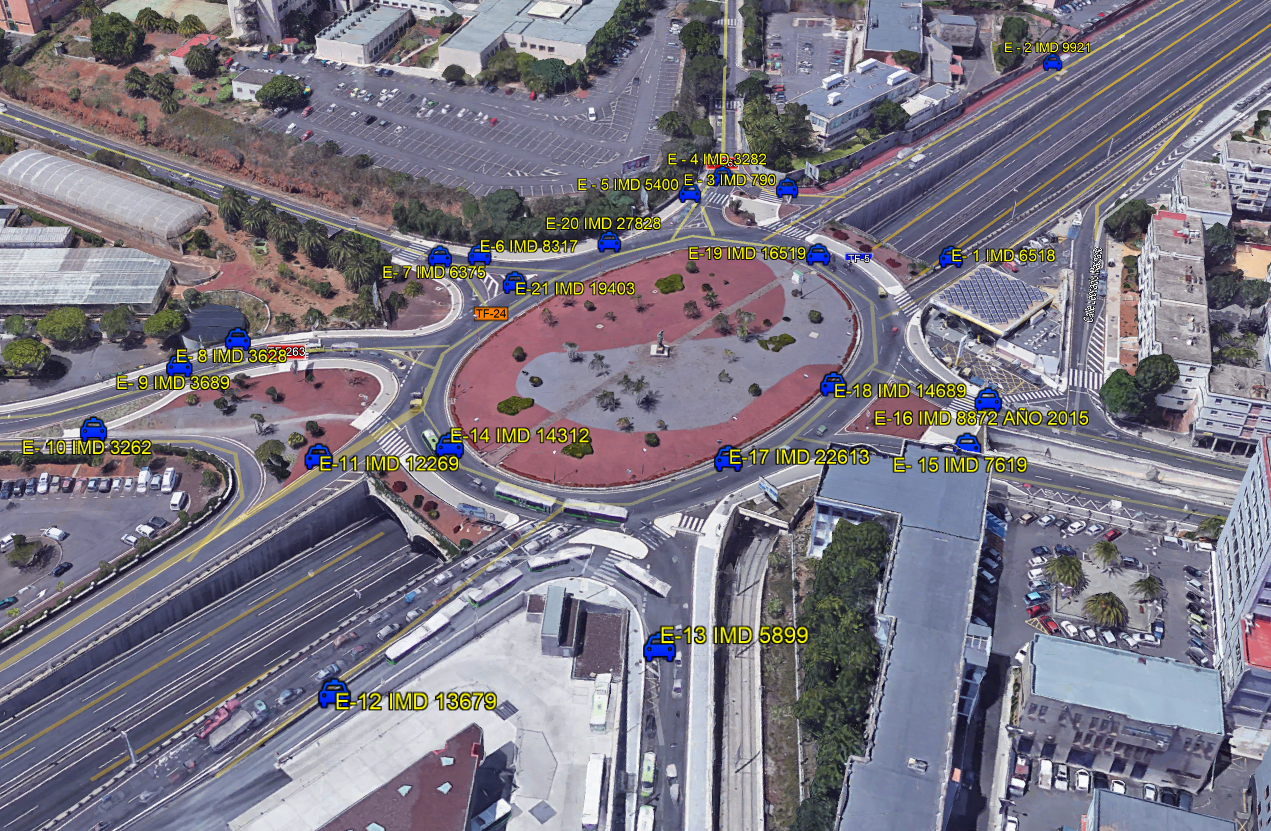
\includegraphics[width=\textwidth]{report/images/aforadores.png}
    \caption{Lugares donde se instalaron los aforadores.}
    \label{fig:aforadores}
\end{figure}

Como nuestro objetivo era simular una hora punta, nos acabamos decantando por obtener los datos del día jueves 21 de noviembre de 2019, a las 8:00, por ser el día que más tráfico hubo a esa hora.

\subsubsection{Generación de rutas: \texttt{flowrouter.py}}

Tener los datos de los aforadores es una gran ayuda a la hora de estimar con fiabilidad el tráfico real de la rotonda, pero no lo es todo, puesto que no indica qué ruta han seguido dichos vehículos ni tampoco cuál es el destino al que habían de llegar. Es decir, es conocido cuántos coches salen de A y cuántos llegan a B, pero no conocemos cuáles de los coches que han llegado a B procedían de A. Al final, de lo que disponemos es de contadores de vehículos, pero lo que nos interesa son las rutas que siguen dichos vehículos; o sea, una matriz O/D.

Así pues, el problema de inferir una matriz O/D a partir de datos de contadores de tráfico no es en absoluto desconocido y abunda bastante literatura sobre cómo abordar este problema (véase~\cite{otto_anker_nielsen_two_1998}). 

Sin embargo, y como no podía ser de otro modo, los creadores de SUMO ya habían previsto que esta situación podría darse, así que decidieron incorporar dos herramientas para calcular las rutas con sus respectivos flujos a partir de datos de aforadores: \texttt{DFROUTER}~\cite{noauthor_dfrouter_nodate}; y su versión mejorada, \texttt{flowrouter.py}~\cite{noauthor_flowrouterpy_nodate,behrisch_route_2018}, la cual ha sido finalmente la empleada para generar el tráfico.

La diferencia entre ambas radica en el algoritmo que emplean para calcular las rutas y los flujos de los vehículos. \texttt{DFROUTER} está pensada para redes en las cuales todas las posibles entradas y salidas cuentan con aforadores, y los datos que estos brindan son relativamente precisos. \texttt{flowrouter.py}, por otro lado, está pensado para trabajar con más incertidumbre y, por tanto, es capaz de lidiar con redes en las cuales faltan aforadores y donde los datos pueden presentar cierto nivel de inconsistencia.

Estas herramientas toman como entrada tres archivos:

\begin{itemize}
    \item El archivo de red.
    \item Un archivo con los datos de los aforadores (nombre, posición, y si es de origen, destino o está <<en medio>> ---esta clasificación, tal y como se infiere de su nombre, está reservada para aforadores que no son clasificables como de origen o destino---).
    \item Datos de flujo (aforador, flujo, plazo durante el cuál se detectó dicho flujo, etc.).
\end{itemize}

Y como salida general dos archivos:

\begin{itemize}
    \item Un archivo de rutas.
    \item Un archivo de flujos (definidos en función de las rutas).
\end{itemize}

Ha de señalarse que ambas herramientas están pensadas para trabajar con redes relativamente simples, concretamente autopistas, dado que suelen estar bien dotadas de aforadores y no poseen una topología especialmente compleja; por lo que es posible que los resultados que brindan dichas herramientas a veces pueden ser erráticos y confusos, por lo que la entrada debe ser lo más completa y precisa posible.

Durante una prueba inicial, los resultados obtenidos con \texttt{flowrouter.py} mostraban que había rutas que no seguía ningún vehículo cuando realmente debía de haber algún flujo. También, en algunos casos, se generaban rutas ilógicas, como circular desde la carretera de Geneto con la intención de incorporarse a la TF-5 sentido sur pasando por la rotonda, ignorando el desvío (más corto) del que dispone la carretera, que permite incorporarse a la autopista directamente.

Es muy posible que este tipo de errores e inexactitudes se produjeran por la intención del algoritmo de satisfacer las restricciones impuestas por los datos de los aforadores. Asimismo, la configuración de algunos de estos contadores no era la idónea. 

Por ejemplo, volviendo al caso de la carretera de Geneto, según muestra la figura~\ref{fig:aforadores}, esta cuenta con tres aforadores: el E-8 (en sentido ascendente), el E-9 (en sentido descendente) y el E-10 (en sentido descendente, colocado en el desvío hacia la autopista).

Se da la circunstancia de que, por la manera en que \texttt{flowrouter.py} calcula las rutas, es posible que designara los orígenes y los destinos en unos nodos en los cuales realmente no deseamos que acabe el tráfico (porque, por ejemplo, no daría tiempo a que se formaran colas o a apreciar mejor durante la simulación el funcionamiento del tráfico).

Todos estos problemas se solucionaron (en su mayoría) añadiendo nuevos contadores manualmente. Para el ejemplo que estamos tratando, bastó con añadir un contador en la carretera de Geneto, sentido descendente, que estuviera un poco más arriba y que sumara el flujo de los contadores E-9 y E-10, y colocando a la misma altura el contador E-8 (el que estaba en sentido ascendente). Hecho con el resto de vías, la generación del tráfico es menos errática y durante la simulación es posible apreciar mejor el flujo de los vehículos.

Este método es, pues, el que mejor resultados ha brindado y es con el que finalmente se llevó a cabo la generación del tráfico.